\documentclass[border=2pt]{standalone}
\usepackage{tikz}
\begin{document}
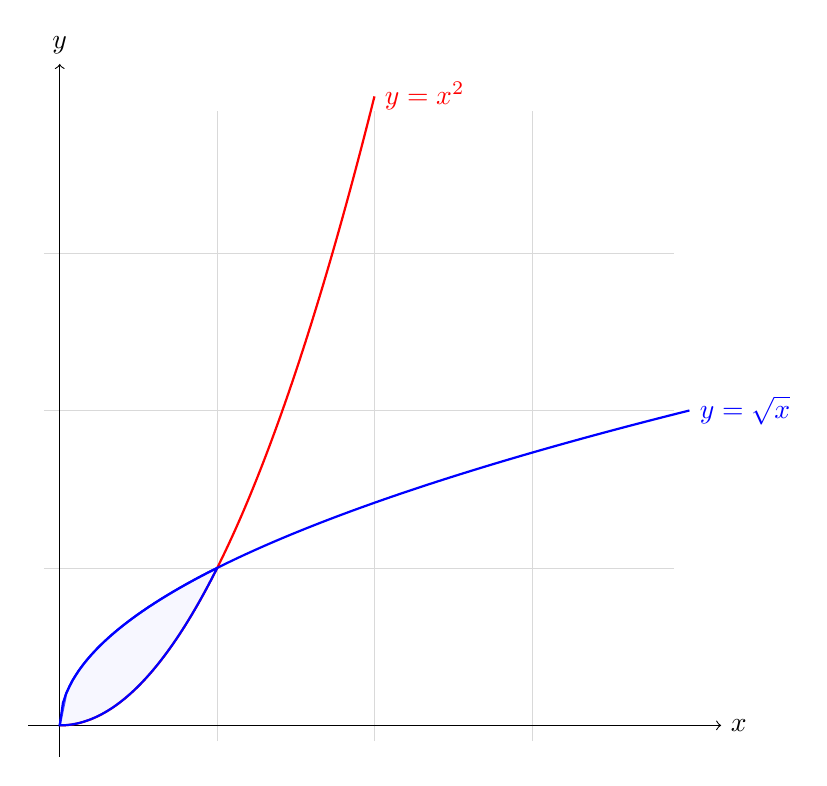
\begin{tikzpicture}[scale=2]
  \draw[very thin, color=gray!30] (-0.1,-0.1) grid (3.9,3.9);
  \draw[->] (-0.2,0) -- (4.2,0) node[right] {$x$};
  \draw[->] (0,-0.2) -- (0,4.2) node[above] {$y$};
  \draw[thick, color=blue] plot[domain=0:4, samples=100] (\x,{sqrt(\x)}) node[right] {$y = \sqrt{x}$};
  \draw[thick, color=red] plot[domain=0:2, samples=100] (\x,{\x*\x}) node[right] {$y = x^2$};
  \filldraw[fill=blue!10, draw=blue, thick, fill opacity=0.3] plot[domain=0:1, samples=50] (\x,{sqrt(\x)}) -- plot[domain=1:0, samples=50] (\x,{\x*\x}) -- cycle;
\end{tikzpicture}
\end{document}
